\documentclass [11pt,twoside]{article}
\usepackage[utf8]{inputenc}
\usepackage[T1]{fontenc}

%Page margins, header and footer positions
\usepackage{geometry}
 \geometry{
 a4paper,
 total={210mm,297mm},
 left=25mm,
 right=25mm,
 top=30mm,
 bottom=25mm,
 headsep=7mm}

\interfootnotelinepenalty=10000

%To display filling dots in the TOC for all entries
\usepackage[titles]{tocloft}
\renewcommand{\cftsecleader}{\cftdotfill{\cftdotsep}}

%Define new header and footer style
\usepackage{fancyhdr}

\pagestyle{fancy}
\fancyhf{}
\lhead{\color{Gray}{\small{SafeStreet Project - Maldini , Paone}}}
\lfoot{\textcolor{Gray}{\small{Copyright © 2019, Maldini, Paone – All rights reserved}}}
\rfoot{\textcolor{Gray}{\thepage}}
\renewcommand{\headrulewidth}{0pt}

%PACKAGES
\usepackage{wasysym}
\usepackage{pifont}

\newcommand{\supported}{\ding{52}\xspace}
\newcommand{\unsupported}{\ding{55}\xspace}
\newcommand{\partsupported}{\textcolor{black!40}{\ding{52}}\xspace}
\newcommand{\lowsupported}{\textcolor{black!20}{\ding{52}}\xspace}
\newcommand{\unknowsupported}{\textbf{?}\xspace}

%Font: Times
\usepackage{times}
%Change monospaced font
\renewcommand{\ttdefault}{lmtt}

%tables
\usepackage{tabu}
\usepackage{tabularx}
\usepackage{ltablex}
\usepackage{longtable}
\usepackage{float} % To allow the use of H modifier in long tables

%landscape mode
\usepackage{pdflscape}
\usepackage{rotating}
\usepackage{caption}

%make landscape mode be sensitive to even and odd pages
%start
\def\myrotate{\ifodd\c@page\else-\fi 90}
\makeatletter
\global\let\orig@begin@landscape=\landscape%
\global\let\orig@end@landscape=\endlandscape%
\gdef\@true{1}
\gdef\@false{0}
\gdef\landscape{%
    \global\let\within@landscape=\@true%
    \orig@begin@landscape%
}%
\gdef\endlandscape{%
    \orig@end@landscape%
    \global\let\within@landscape=\@false%
}%
\@ifpackageloaded{pdflscape}{%
    \gdef\pdf@landscape@rotate{\PLS@Rotate}%
}{
    \gdef\pdf@landscape@rotate#1{}%
}
\let\latex@outputpage\@outputpage
\def\@outputpage{
    \ifx\within@landscape\@true%
        \if@twoside%
            \ifodd\c@page%
                \gdef\LS@rot{\setbox\@outputbox\vbox{%
                    \pdf@landscape@rotate{-90}%
                    \hbox{\rotatebox{90}{\hbox{\rotatebox{180}{\box\@outputbox}}}}}%
                }%
            \else%
                \gdef\LS@rot{\setbox\@outputbox\vbox{%
                    \pdf@landscape@rotate{+90}%
                    \hbox{\rotatebox{90}{\hbox{\rotatebox{0}{\box\@outputbox}}}}}%
                }%
            \fi%
        \else%
            \gdef\LS@rot{\setbox\@outputbox\vbox{%
                \pdf@landscape@rotate{+90}%
                \hbox{\rotatebox{90}{\hbox{\rotatebox{0}{\box\@outputbox}}}}}%
            }%
        \fi%
    \fi%
    \latex@outputpage%
}
\makeatother
%end

%graphics
\usepackage{graphicx}
\usepackage[dvipsnames, table]{xcolor}
%If you upload images from PC, you need to insert code for the path here (different for Windows and Unix OS)

%References
%\usepackage{xpatch}
%\usepackage[backend=biber, style=numeric, citestyle=numeric, sorting=none]{biblatex}
%\addbibresource{main.bib}

%Other
\usepackage{ifthen}
\usepackage{xspace}
\usepackage{enumitem}
\usepackage{amssymb}
\usepackage[pdftex, colorlinks]{hyperref}
\newcommand{\comment}[1]{{\color{Red}$\blacktriangleright$ Comment: #1 $\blacktriangleleft$}}


% Some utilities\ldots
\usepackage{soul}
\usepackage{tikz}

\usetikzlibrary{calc}
\usetikzlibrary{decorations.pathmorphing}


\makeatletter

\newcommand{\defhighlighter}[3][]{%
  \tikzset{every highlighter/.style={color=#2, fill opacity=#3, #1}}%
}

\defhighlighter{yellow}{.5}

\newcommand{\highlight@DoHighlight}{
  \fill [ decoration = {random steps, amplitude=1pt, segment length=15pt}
        , outer sep = -15pt, inner sep = 0pt, decorate
       , every highlighter, this highlighter ]
        ($(begin highlight)+(0,8pt)$) rectangle ($(end highlight)+(0,-3pt)$) ;
}

\newcommand{\highlight@BeginHighlight}{
  \coordinate (begin highlight) at (0,0) ;
}

\newcommand{\highlight@EndHighlight}{
  \coordinate (end highlight) at (0,0) ;
}

\newdimen\highlight@previous
\newdimen\highlight@current

\DeclareRobustCommand*\highlight[1][]{%
  \tikzset{this highlighter/.style={#1}}%
  \SOUL@setup
  %
  \def\SOUL@preamble{%
    \begin{tikzpicture}[overlay, remember picture]
      \highlight@BeginHighlight
      \highlight@EndHighlight
    \end{tikzpicture}%
  }%
  %
  \def\SOUL@postamble{%
    \begin{tikzpicture}[overlay, remember picture]
      \highlight@EndHighlight
      \highlight@DoHighlight
    \end{tikzpicture}%
  }%
  %
  \def\SOUL@everyhyphen{%
    \discretionary{%
      \SOUL@setkern\SOUL@hyphkern
      \SOUL@sethyphenchar
      \tikz[overlay, remember picture] \highlight@EndHighlight ;%
    }{%
    }{%
      \SOUL@setkern\SOUL@charkern
    }%
  }%
  %
  \def\SOUL@everyexhyphen##1{%
    \SOUL@setkern\SOUL@hyphkern
    \hbox{##1}%
    \discretionary{%
      \tikz[overlay, remember picture] \highlight@EndHighlight ;%
    }{%
    }{%
      \SOUL@setkern\SOUL@charkern
    }%
  }%
  %
  \def\SOUL@everysyllable{%
    \begin{tikzpicture}[overlay, remember picture]
      \path let \p0 = (begin highlight), \p1 = (0,0) in \pgfextra
        \global\highlight@previous=\y0
        \global\highlight@current =\y1
      \endpgfextra (0,0) ;
      \ifdim\highlight@current < \highlight@previous
        \highlight@DoHighlight
        \highlight@BeginHighlight
      \fi
    \end{tikzpicture}%
    \the\SOUL@syllable
    \tikz[overlay, remember picture] \highlight@EndHighlight ;%
  }%
  \SOUL@
}

\makeatother

% Common abbrev. are set as commands to ensure proper spacing after the dot
\RequirePackage{xspace}
\newcommand{\ie}{i.e.\@\xspace}
\newcommand{\aka}{a.k.a.\@\xspace}
\newcommand{\Ie}{I.e.\@\xspace}
\newcommand{\cf}{cf.\@\xspace}
\newcommand{\Cf}{Cf.\@\xspace}
\newcommand{\eg}{e.g.\@\xspace}
\newcommand{\Eg}{E.g.\@\xspace}
\newcommand{\etal}{et al.\@\xspace}
\newcommand{\etc}{etc.\@\xspace}
\newcommand{\wrt}{w.r.t.\@\xspace}
\newcommand{\Wrt}{W.r.t.\@\xspace}



\date{}

\usepackage{bookmark}
\usepackage{placeins}
\let\Oldsection\section
\renewcommand{\section}{\FloatBarrier\Oldsection}
\let\Oldsubsection\subsection
\renewcommand{\subsection}{\FloatBarrier\Oldsubsection}
\let\Oldsubsubsection\subsubsection
\renewcommand{\subsubsection}{\FloatBarrier\Oldsubsubsection}
\usepackage{eso-pic,graphicx}
\usepackage[top=2cm, bottom=2cm, outer=0cm, inner=0cm]{geometry}


\begin{document}

%TITLE PAGE

\begin{titlepage}


%LOGO

{\begin{table}[t!]
\centering
\begin{tabu} to \textwidth { X[1.3,r,p] X[1.7,l,p] }
\textcolor{Blue}
{\textbf{\small{Computer science and engineering Software engineering 2 - Project 2019/2020}}} & 
\includegraphics[scale=0.5]{Images/PolimiLogo}
\end{tabu}
\end{table}}~\\ [7cm]
%TODOour logo

%TITLE 

\begin{flushleft}



\end{flushleft}
\AddToShipoutPictureBG*{
\includegraphics[width=\paperwidth,height=\paperheight]{Images/SafeStreets.png}}
\end{titlepage}


\begin{table}[h!]
\begin{tabu} to \textwidth { X[0.3,r,p] X[0.7,l,p] }
\hline

\textbf{Deliverable:} & RASD\\
\textbf{Title:} & Requirement Analysis and Verification Document \\
\textbf{Authors:} & Maldini Pietro , Paone Angelo \\
\textbf{Version:} & 1.0 \\ 
\textbf{Date:} & 10-November-2019 \\
\textbf{Download page:} & https://github.com/pm390/MaldiniPaone\\
\textbf{Copyright:} & Copyright © 2019, Maldini Pietro, Paone Angelo – All rights reserved \\
\hline
\end{tabu}
\end{table}




\setcounter{page}{2}


%------------------------------------------------------------------------------------------------------------------------------------------------
\newpage
\addcontentsline{toc}{section}{Table of Contents}
\tableofcontents


%------------------------------------------------------------------------------------------------------------------------------------------------
\clearpage
{\color{Blue}{\section{Introduction}}}
\label{sect:introduction}

%---------------------------------------------------
\subsection{Purpose}
This document represents the Requirement Analysis and Specification Document (RASD). Goals of
this document are to completely describe the system-to-be in terms of functional and non-functional
requirements, analyse the real needs of the users in order to model the system, show the constraints
and the limit of the software and indicate the typical use cases that will occur after the release. This
document is addressed to the developers who have to implement the requirements and could be used as
a contractual basis. 
%---------------------------------------------------
\subsubsection{Goals}
\begin{itemize}
\item	USER:
\begin{itemize}
\item[G1] Notify authorities about traffic violations
\begin{itemize}
\item[G1-1] Send picture of violation
\item[G1-2] Send Position of the violation
\end{itemize}
\item[G2]Authorities must be able to take an available assignment
\item[G3] Allow authorities to report a finished assignment
\item[G4]Allow all actors to visualize update statistics
\item[G5] Allow the system manager to register Municipality to the service
\end{itemize}
\item	SafeStreets:
\begin{itemize}
\item[G6] Allow a Visitor to join the system registering him/herself to ensure reliability of the information provided by him/her
\item[G7] Store information about violations provided by users:
\begin{itemize}
\item[G7-1] Complete it with metadata
\item[G7-2] Mine information
\end{itemize}
\item[G8] Identify potentially unsafe areas:
\begin{itemize}
\item[G8-1] Suggest possible interventions
\end{itemize}
\item[G9] Allow municipality to register Authorities to the service
\end{itemize}
\item	Security Goals:
\begin{itemize}
\item[S1] Offer different levels of visibility to different type of users
\item[S2] Personal data of users are stored respecting current security standards
\end{itemize}
\end{itemize}
%---------------------------------------------------
\subsection{Scope}
\subsubsection{Description of the given problem}
SafeStreets is a crowd-sourced application whose intention is to notify the authorities when traffic
violations occur. Citizens, thanks to the system, will be able to send information about violations to the
authorities who will take actions against them. In this way, the service provided by the authorities can be
improved because they will receive notifications through the app. The sources of notifications are the
Citizens who take photos of violations and send them to the authorities through
the application. The information provided by users are integrated with other suitable information and are
stored by the service. The system also runs an algorithm to read the license plate of the vehicle in the
photos. All collected data can be seen by Citizens and authorities to find which streets are the safest.
Users can have different levels of visibility: authorities must be able to know the license plates of vehicles
in the photos, while normal users can only see data in the form of statistics. Moreover, data are sent to
the municipal district so that important information can be extracted through statistics in order to make
decisions to improve the safety of the area. Finally, the system will have to be easy to use, reliable
and highly scalable to fit perfectly with the mutable context in which it will be used.

%---------------------------------------------------
\subsubsection{Phenomena}
\begin{itemize}
\item
World phenomena:
\begin{enumerate}
\item
Violation
\item
Intervention of authorities
\item
Municipality put into effect interventions to improve safety
\end{enumerate}
\item
Machine phenomena:	
\begin{enumerate}
\item
Shortest path calculation for authority’s intervention (done by mapping system)
\item
the creation of an object of type violation
\item
run algorithm to identify the license plate/s in the photos
\item
schedule most efficient path to look up the notified violations
\item
periodically run algorithm to suggest possible interventions to municipality
\end{enumerate}
\item
Shared phenomena:
\begin{enumerate}
\item
user notify the system about violation (observed by the system controlled by the world)
\item
send notification to authorities (controlled by system observed by world)
\end{enumerate}
\end{itemize}
%---------------------------------------------------
\subsection{Definitions, Acronyms, Abbreviations}
\subsubsection {Definitions}
\begin{itemize}
\item	Violation: parking violations which can be notified by Citizens to authorities
\item	Report: Notification sent by Citizens to the system
\item	Mapping System: external software that provides maps and directions to reach the position of a violation
\item	Licence plate Recognition Algorithm: calculation process that identifies the alphanumeric number on license plate
\item	Spam: a series of messages that are undesired
\item	App: application software 
\item	Blocked: means that the account is banned for a given period
\item	Metadata: data about a violation. Position , date,  time and the username of Citizen. 
\item	Assignment : Work Request for authorities generated upon the receiving of a notification made by Citizens.
\end{itemize}
%---------------------------------------------------
\subsubsection {Acronyms}
\begin{itemize}
\item	RASD: Requirement Analysis and Specification Document.
\item	API: Application Programming Interface
\item	GPS: Global positioning system
\item	HTTP: HyperText Transfer Protocol
\item	HTTPS: HyperText Transfer Protocol over Secure Socket Layers
\item	UML: Unified Modeling Language

\end{itemize}
%---------------------------------------------------
\subsubsection {Abbreviations}
\begin{itemize}
\item	[Gn]: n-th goal.
\item	[Dn]: n-th domain assumption.
\item	[Rn]: n-th requirement.
\item     Municipality: municipal employee.
\end{itemize}
%---------------------------------------------------
\subsection {Revision History}
\begin{itemize}
\item      RASDv1.0 felivered on 10/11/2019: first delivery.
\item	RASDv2.0 delivered on 15/12/2019 : TODO write what we modified
\end{itemize}
%---------------------------------------------------
\subsection {Reference Documents}
\begin{itemize}
\item	Specification Document: “Assignments AA 2019-2020.pdf”.
\item	\href{http://homepage.cs.uiowa.edu/~tinelli/classes/181/Spring10/Notes/09-dynamic-models.pdf }{Alloy Dynamic Model example} 
\item	IEEE Std 830-1993 - IEEE Guide to Software Requirements Specifications.
\item	IEEE Std 830-1998 - IEEE Recommended Practice for Software Requirements Specifications.

\end{itemize}
%---------------------------------------------------
\subsection{Document Structure}
This chapter debates about contents and structure of RASD, indeed this document, based on standards IEEE, is divided in six different sections:
\begin{enumerate}
\item	The Introduction provides a general appearance of the systems defining which are the goals to reach, describing the problem and introducing the world and shared phenomena.
\item The Overall Description provides the description of the relevant components that system needs, the involved actors’ characteristics, and the assumptions to better clarify the needs and the boundaries of the system. 
\item Specific Requirements contains the goals, the functional and non-functional requirements of the system are presented. In addition, a mock-up representation of the application expslain and gives a feeling on how the app will look like and show the main actions it can perform.
\item Scenarios describe the usefulness of SafeStreet and its features in some situations that could happen.
\item UML Modelling contains the diagrams that are referred to the functionality of the system, they explain the workflow of some scenarios, the actions and the structure of the actors and the state that system assumes. These features are represented by Use Case diagram, Sequence diagram, Class diagram and Activity diagram.
\item Alloy Modelling allows to explain the world models through Alloy model of system. The mockups generated by the Alloy modelling grants that, given requirements and domain assumption, the goals are satisfied.

\end{enumerate}


%------------------------------------------------------------------------------------------------------------------------------------------------
\clearpage
{\color{Blue}{\section{Overall Description}}}
\label{sect:overview}
\subsection{Product perspective}
The system will be developed from scratch using external elements such as Mapping systems and algorithm to recognise licence plates. We choose to take those external elements to decouple mapping problems from our project implementation and to use already tested algorithms to recognise licence plates.
\subsubsection{Further analysis on shared phenomena}
\subsubsection{Class Diagram}
\begin{figure}[h]
\centering
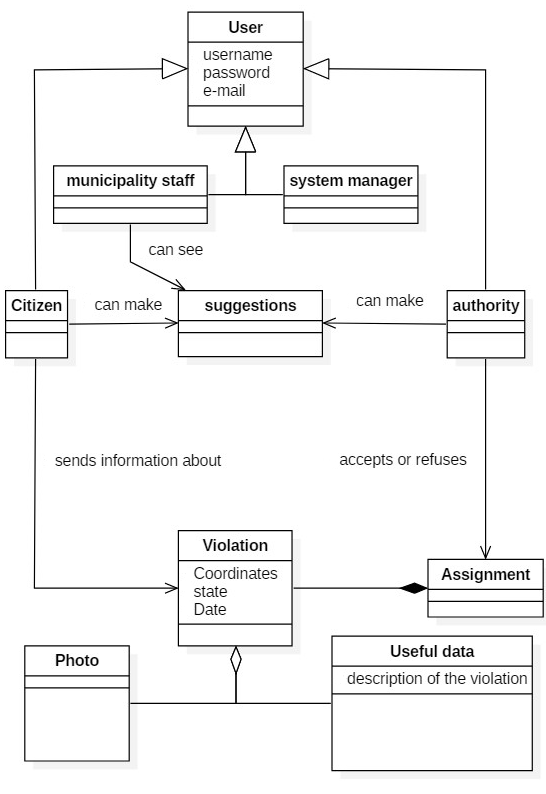
\includegraphics{Images/classdiagram.png}
\caption{\label{fig:cs} Class Diagram}
\end{figure}
\newpage
\subsubsection{Statechart report}
\begin{figure}[h]
\centering
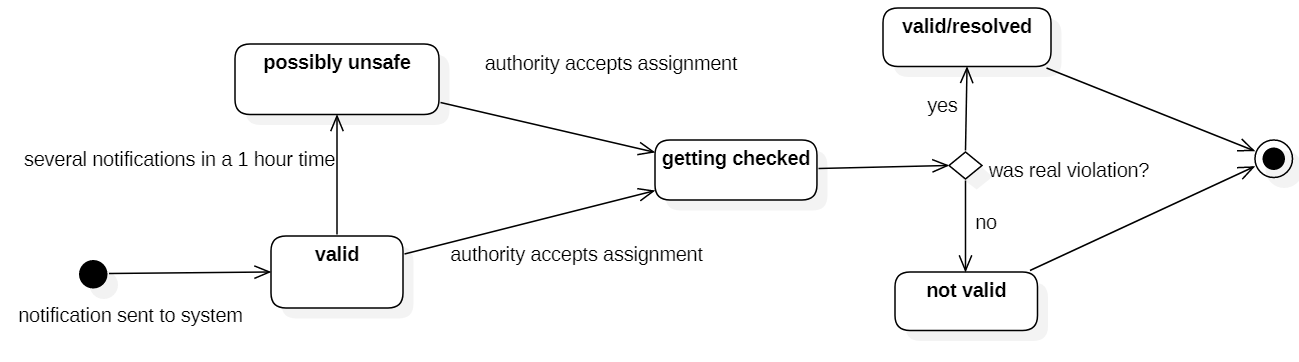
\includegraphics[width=\textwidth]{Images/statechartreport.png}
\caption{\label{fig:sc1} Statechart report}
\end{figure}
\subsubsection{Statechart assignment}
\begin{figure}[h]
\centering
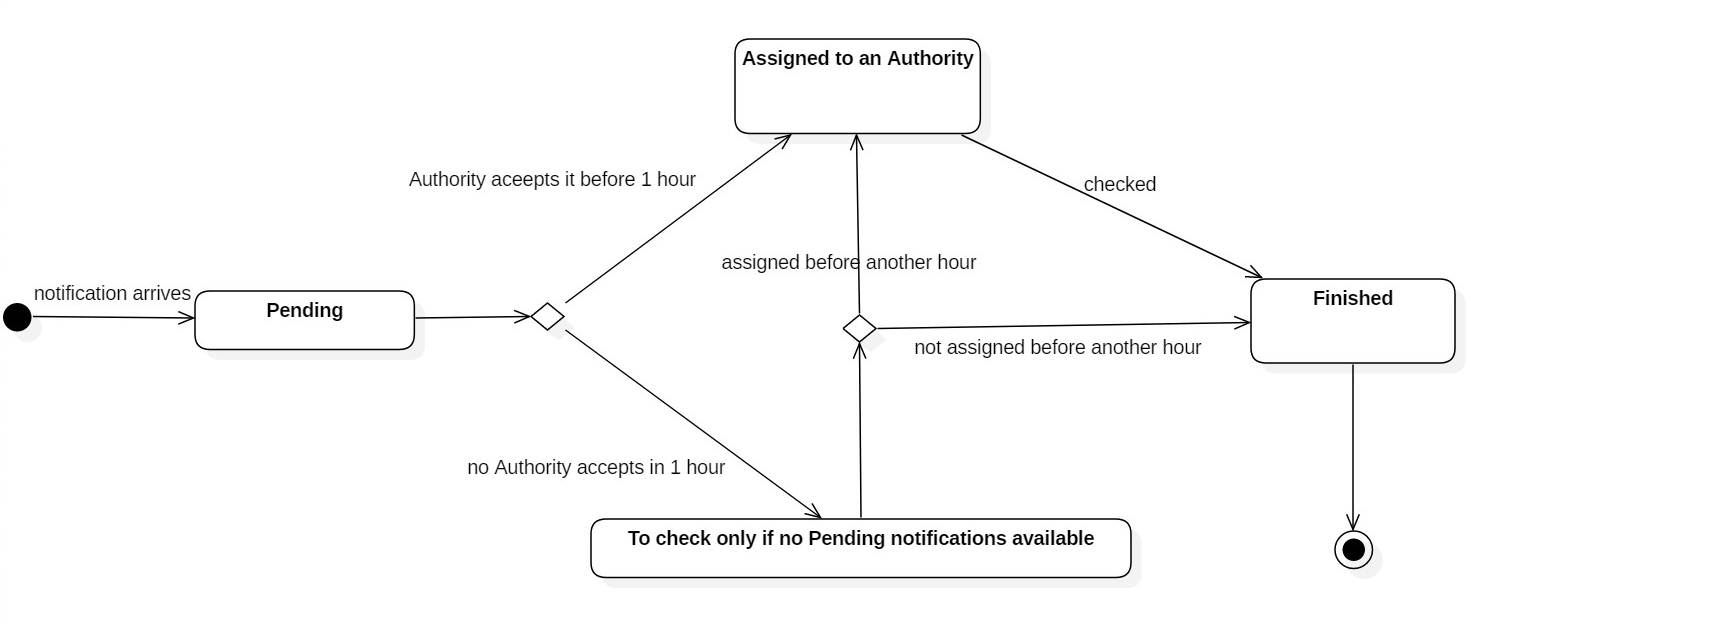
\includegraphics[width=\textwidth]{Images/statechartassignment.png}
\caption{\label{fig:sc2} StateChart assignment}
\end{figure}



%---------------------------------------
\subsection{Product functions}
In this section we provide a list of functionalities offered by our system. We will describe those functionalities and in later section we will better analyse interactions of users with those functions.
\subsubsection{ Mapping System }
An external mapping system will be used to guarantee better performances than a system to implement from scratch.
This won’t ensure always the correctness of information given by that system. Some issues about mapping systems like accidents occurred and blocked streets can’t be addressed in real time. Those kinds of problems may need to rely on authority’s knowledge of the area to be overcome.
\subsubsection{Licence Plate Recognition Algorithm}
An external Licence Plate recognition algorithm will be adopted in our system. There are a lot of services provided online and some open-source solutions. Those systems are used by several people and companies and are tested so most kind of issues that may occur has already been noticed and fixed. Considering our system is to be launched in Italy we will consider a solution better suited to recognize European licence plates.
\subsubsection{Municipality Servers maintenance}
Our system can’t address problem of municipality server’s unavailability issues. If a server is unavailable and needs maintenance statics for the area covered by that server may become unavailable for an indefinite amount of time. To solve this problem SafeStreets may use the email address used to register the municipality to contact it and to point out the issues.
%---------------------------------------
\subsection{Actors characteristics}
\begin{itemize}
\item Visitor: a person using SafeStreets without being registered. He/she can only see statics, register or sign-in to be recognized as a User
\item Registered User/ User: term used to identify any person which uses our application and has registered to our service:
\item  Citizen: Is a User who provide the system information and are the main contributors to the service. They provide information about violations with photos and possibly some notes. They can access data gathered by the system in form of statistics.
\item Municipality: Users managing local systems in each area. Those users should be able to take decisions to change unsafe areas thanks to their status.
\item Authority: police agents. They are invited to use the service by municipality users who can ask creation of their account. They can reserve assignments of violations to be addressed. They can also refuse the assignment, mark it as spam or send it to another authority.
\item System Manager: User who is responsible of the system, therefore he/she has all the possible privileges to manage the system.For example he/she can register a new municipality
\end{itemize}
%---------------------------------------
\subsection{Assumptions, dependencies and constraints}
\subsubsection {Regulatory policies}
The system will ask user for minimal information to recognize them. The visitor should give the system only his /her email address and provide the system a username and a password to create an account. Email addresses won’t be used for commercial uses and will be stored only to give the possibility to recover an account in case the user loses his/her credentials.
\subsubsection{ Interfaces to other applications}
In the first release no public interfaces will be opened and SafeStreets will only communicate with municipality servers to retrieve useful information about accidents.
\subsubsection{ Domain assumptions}
\begin{itemize}
\item D1) For each notification data and metadata about the violation are correct
\item D2) Each Username is unique
\item D3) Authorities always intervene in case of a notified violation
\item D4) Information about authorities’ location are always available through GPS 
\item D5) Only agents close to the violation area are notified 
\item D6) Citizen sends only clear photos (if it is not clear he/she would retake the photo)
\item D7) System Manager, Municipality and authorities respects their duty of care
\item D8) When an authority is sent an email to register this will surely be received
\item D9) Information provided by authority are correct and no false report is ignored (always reported by authority as false).
\item D10) Citizens’ Location are retrieved by GPS or manual input and are correct
\item D11) The Agent must be contactable from municipality  
\item D12) Information of authority are known by municipality
\item D13) Information provided from Users must be correct
\end{itemize}


%------------------------------------------------------------------------------------------------------------------------------------------------
\clearpage
{\color{Blue}{\section{Specific Requirements}}}
\label{sect:requirements}
%.-------------------------------------------------------------------------------------------------------------------------------------------------------------
\subsection{External Interface Requirements}
%.-------------------------------------------------------------------------------------------------------------------------------------------------------------
\subsubsection{User Interfaces}


\begin{figure}[h]
\centering
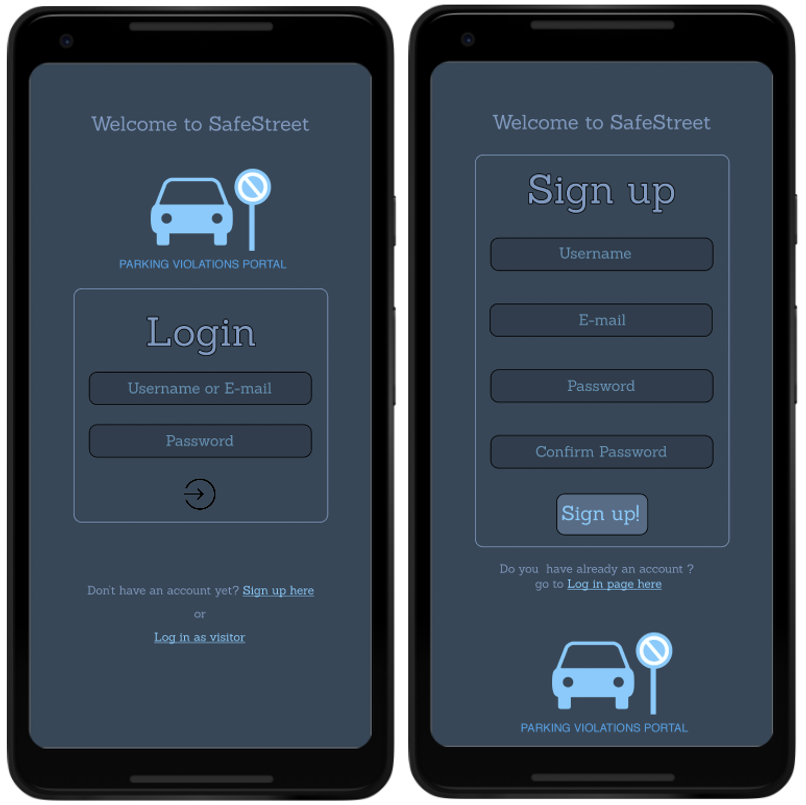
\includegraphics[width=\textwidth]{Images/login_signup.png}
\caption{\label{fig:ls}Login and Sign up }
\end{figure}

\begin{figure}[h]
\centering
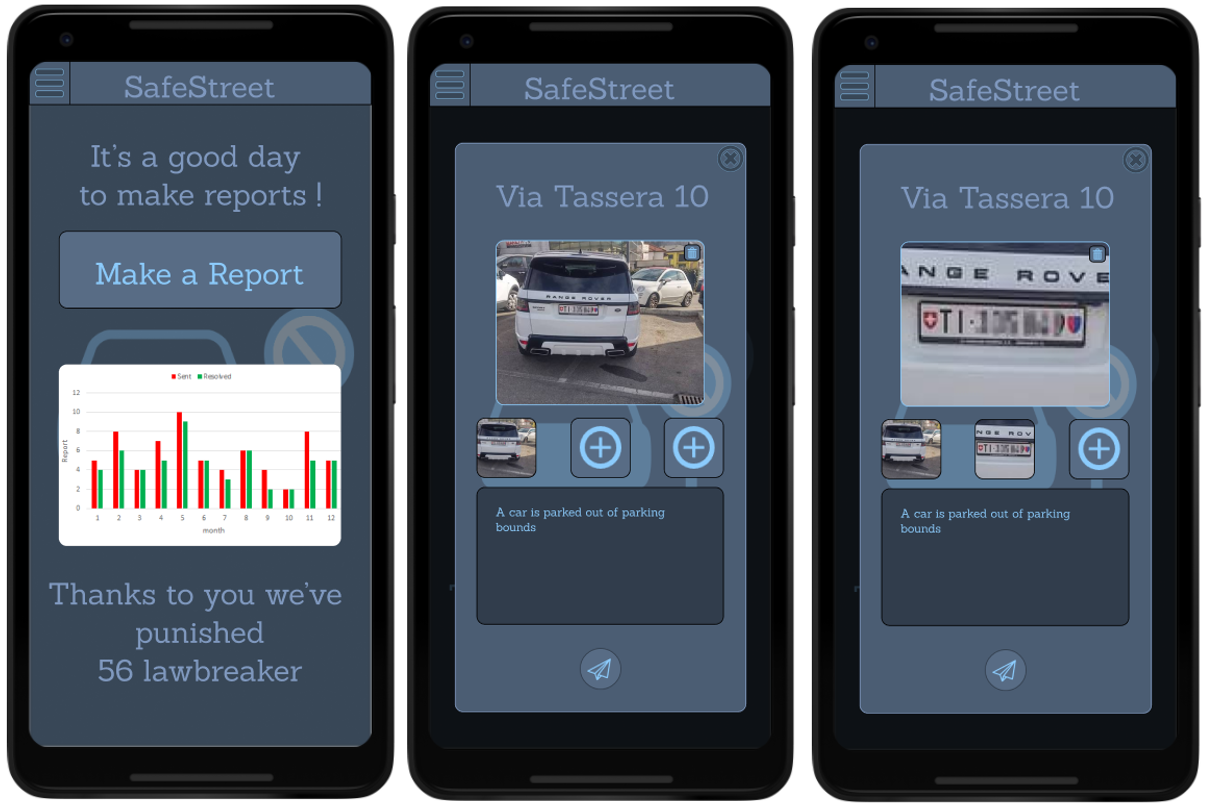
\includegraphics[width=\textwidth]{Images/user_interface.png}
\caption{\label{fig:CI}Citizen Interfaces}
\end{figure}

\begin{figure}[h]
\centering
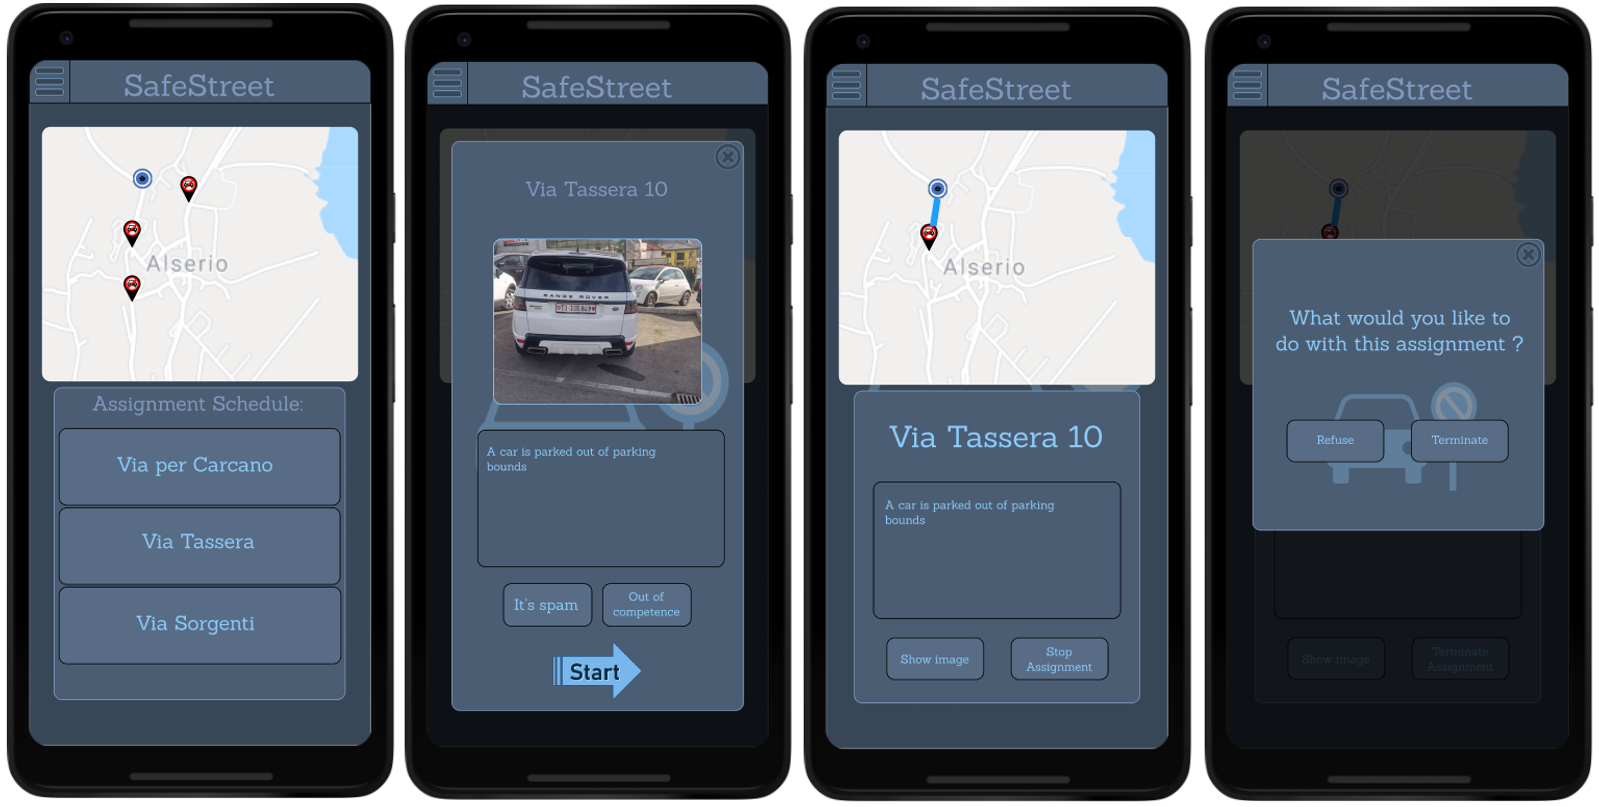
\includegraphics[width=\textwidth]{Images/agent_interface.png}
\caption{\label{fig:AI}Authority Interfaces }
\end{figure}

\begin{figure}[h]
\centering
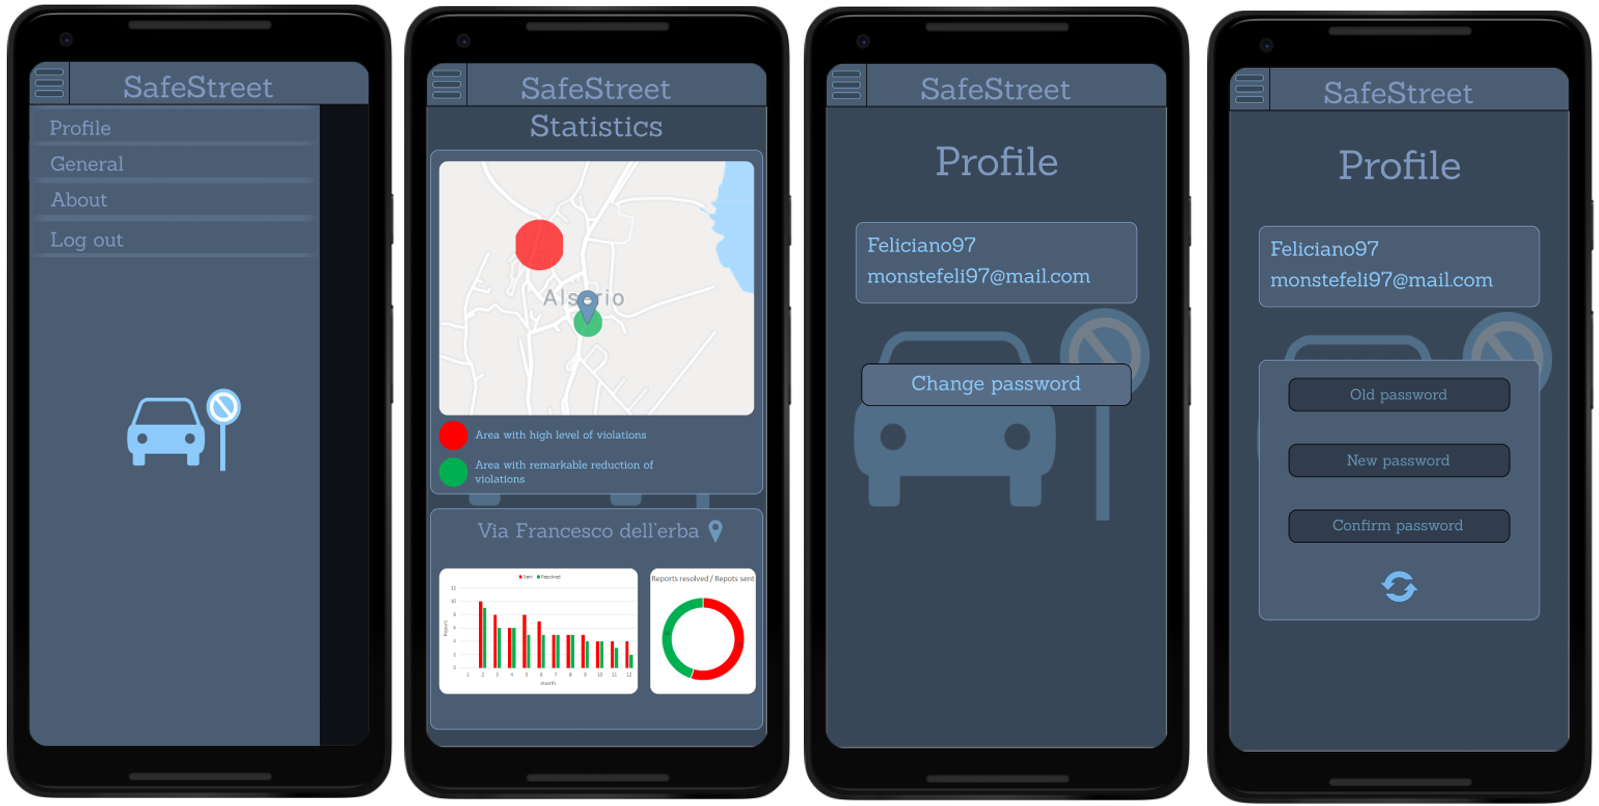
\includegraphics[width=\textwidth]{Images/common_interface.png}
\caption{\label{fig:ComI}Common Interfaces }
\end{figure}

\begin{figure}[h]
\centering
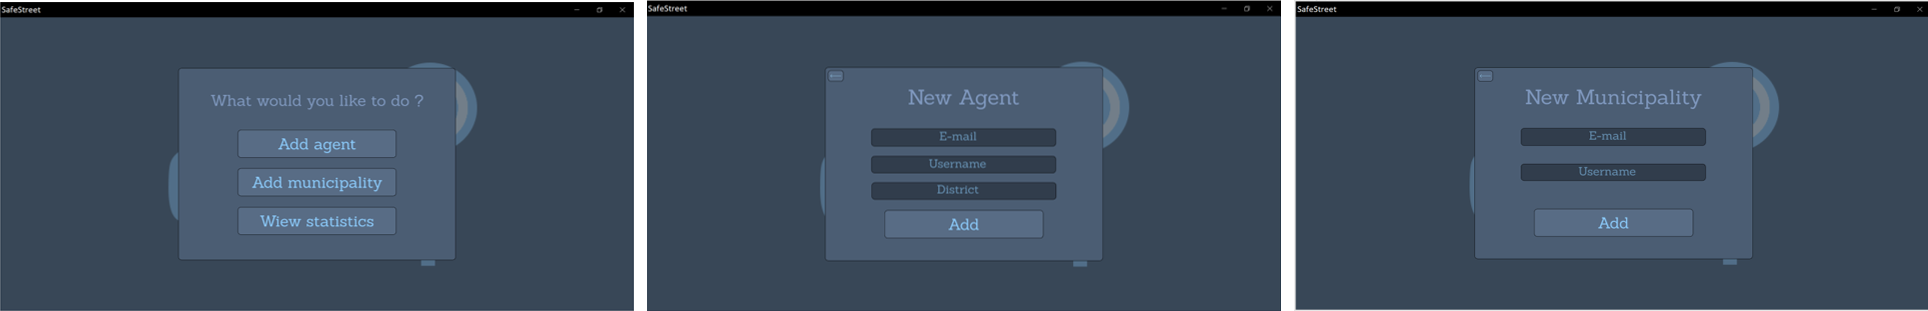
\includegraphics[width=\textwidth]{Images/municipality_interface.png}
\caption{\label{fig:MI}Municipality Interfaces }
\end{figure}

\begin{figure}[h]
\centering
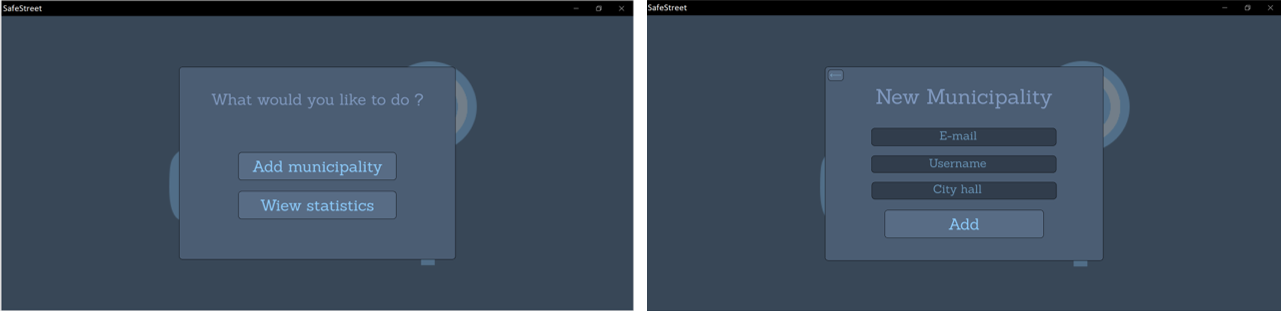
\includegraphics[width=\textwidth]{Images/system_manager_interface.png}
\caption{\label{fig:SMI}Sytem Manager Interfaces}
\end{figure}

\begin{figure}[h]
\centering
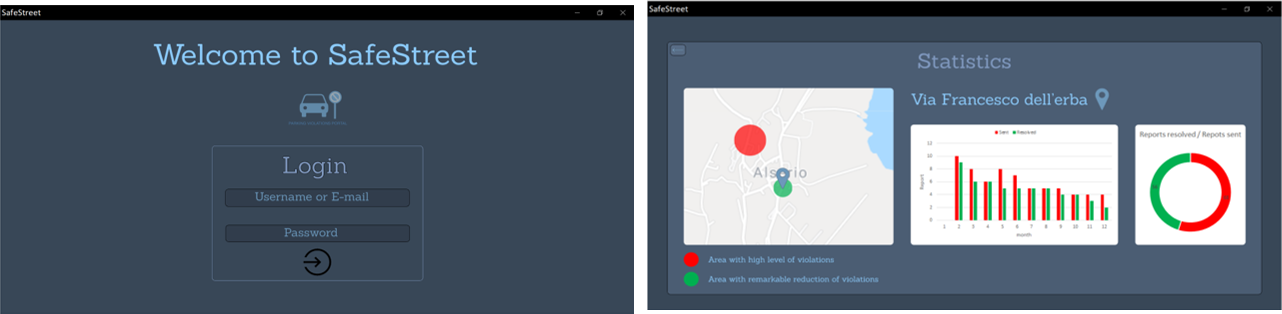
\includegraphics[width=\textwidth]{Images/desktop_common_interface.png}
\caption{\label{fig:ComWI}Common web Interfaces}
\end{figure}

%.-------------------------------------------------------------------------------------------------------------------------------------------------------------
\subsubsection{Hardware Interfaces}
There are no hardware interfaces to be implemented
%.-------------------------------------------------------------------------------------------------------------------------------------------------------------
\subsubsection{Software Interfaces}
Software interfaces to communicate with mapping systems, municipality databases and the algorithm to read Lisence plates are needed 
%.-------------------------------------------------------------------------------------------------------------------------------------------------------------
\subsubsection{Communication Interfaces }
To communicate the various internal parts of the S2B use HTTP and HTTPS protocol. No specific communication interface must be implemented.
%.-------------------------------------------------------------------------------------------------------------------------------------------------------------
\subsection{Functional Requirements}
\begin{itemize}

 \item R1) Authorities’ location must be known by the system when they are in service.
\item  R2) When a Citizen makes a report the position is correctly added with the GPS when is available.
\item R3) The right authorities are notified about violations.
 \item R4)  Authority must be able to provide the system how the assignment finished: resolved and the type of violation, no intervention needed when arrived, false report.
 \item R5) The system must make Statistics available when asked.
 \item R6) Statistics are always updated when an event happens.  
\item R7) For registering a Municipality his/hers data must be provided to a System manager who will add those data to the service to sign up him/her.
 \item R8) A visitor must be able to begin sign up process in the SafeStreets App filling a form with his data.
 \item R9) When the creation of an account is successful the system must notify the Visitor sending an email to the address provided in the sign up process. 
 \item R10) When GPS is not available the user can input the position from a map.
 \item R11) Users to use the full service must be able to login providing the right credentials.
\item R12) The camera of the mobile phone must be accessible to take photos of violations.
\item R13) Suggestions must be available when municipalities requests them.
\item R14) The User must be able to select the licence plate between the ones in output from the Licence Plate Recognition algorithm.
\item R15) Each Username is unique
\end{itemize}
%.-------------------------------------------------------------------------------------------------------------------------------------------------------------
\subsubsection{Scenrarios}
\begin{itemize}
\item Scenario 1:
\newline
Dimitri has an important appointment, but in front of his underground garage there is a car parked that doesn’t allow him to go out. He doesn’t know who the car owner is, so he can’t call him to move it. So, Dimitri decides to use Safestreet application: he takes a photo of the car, he adds the notes and he insert manually the position, because the GPS can’t take correctly the position, in order to send the violation to the authorities. After 10 minutes the public security agent, who has received the notification of Dimitri’s alert, arrives and means of removal take the car away and finally Dimitri can go to the appointment.


\item Scenario 2:
\newline
Angelo is the town councilman of Alserio. In the last period some citizen has alerted him that there are some people who park their car in the disabled parking near the Enigma café. They also have complained about the fact that there is not a public security agent to control the area. So, Angelo asks the mayor to use SafeSteets application in order to keep the violations under control. The mayor, enthusiast of his suggestion asks the system manager to add him into the service.After that, the mayor adds the other municipality employees, so they can add the authorities too.Therefore , thanks to the app , the authorities receive warnings about infractions in various part of the town and they can intervene. Moreover, thanks to the statistics supplied by the application, the mayor manages to start a policy of prevention of the violation.
\item Scenario 3
\newline
Manuel asks his friend Fred if he wants to join him for dinner this evening at his place. Unfortunately, Fred's car is blocked by a vehicle parked in front of his garage. He has noticed that car has been there several days in the past months. Since Fred works near his house, he goes to work by bike, but his friend lives far from his house, so he can't get there without his car. So, Fred decides to download SafeStreets app on his smartphone. He provides all the information required to the system in order to sign up; then he logs in and sends a notification to the authorities. One hour before leaving he notices that the car has been removed. From that day on the car owner stopped parking there.
\item Scenario 4:
\newline
Today in Milan there are lot of violations and the authorities can't check every one of them. After some time, the violations not assigned lose their priority and go down in the assignment list. Agent Carlo usually checks the areas between Milano Piola and Milano Lambrate. Lots of violations are notified by users in those areas. However, by the time he finishes checking some violations, other become less visible due to the great amount of notifications. When different users notify a violation concerning a license plate in the same area, this one becomes more visible in the assignment list. Thanks to this feature, Carlo is able to first address issues affecting more people.

\item Scenario 5:
\newline
Pietro is an agent who has just been employed in Alserio police; his method of street controlling is “old school” and a little bit disorganized, but his colleague Sonia recommends him SafeStreet application. So, Pietro goes to the town hall to register himself into the Safestreet database. The employee checks his credential and his work district, and the system sends him the transient credential.  Then, Pietro installs the app and uses the transient credentials in order to log into his personal page and change the credentials to confirm the account. Thanks to SafeStreet application, his job is now organized better because he can go to exact violations place.
\item  Negative Use Scenario 6:
\newline
Fernand got his car fined after having parked in a forbidden area. He has been doing it for years, but now he notices that people in that area started using SafeStreets app and thinks that he was fined because of it instead of his behaviour. He decides to "take revenge" subscribing to the app and sending several false notifications. Since he has sent several random photos without any visible licence plate, the system signs the assignments given by Fernand account as "possibly unsafe". After that some agents have checked that no violation is actually in any of the photos sent to the system, his account gets blocked and Fernand can no longer interfere with the normal activities of authorities using the app. After being blocked, Fernand stops complaining about the app and a week later he finds a parking area to replace his former parking spot.
\end{itemize}
%.-------------------------------------------------------------------------------------------------------------------------------------------------------------
\newpage
\subsubsection{Use Case Diagrams}
\begin{figure}[h]
\centering
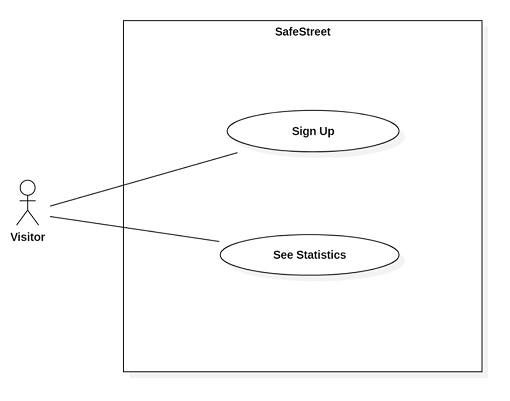
\includegraphics{Images/usecase_visitor.png}
\caption{\label{fig:VUC}Visitor Use Case }
\end{figure}
\begin{figure}[h]
\centering
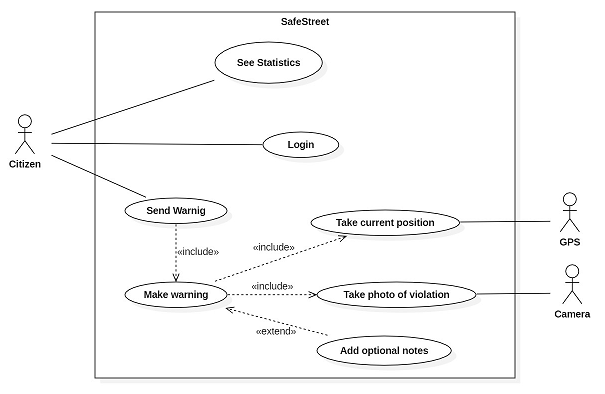
\includegraphics[width=\textwidth]{Images/usecase_citizen.png}
\caption{\label{fig:CUC}Citizen Use Case }
\end{figure}
\begin{figure}[h]
\centering
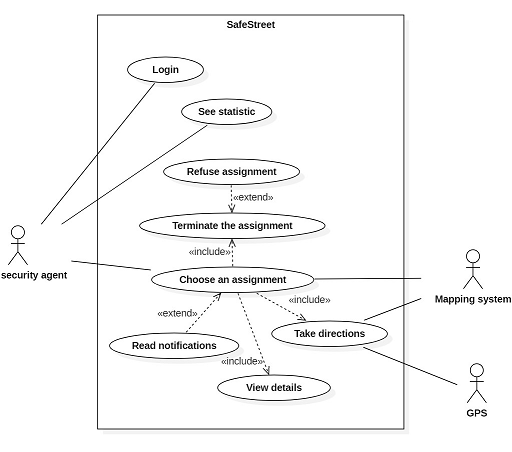
\includegraphics{Images/usecase_agent.png}
\caption{\label{fig:AUC}Authority Use Case }
\end{figure}
\begin{figure}[h]
\centering
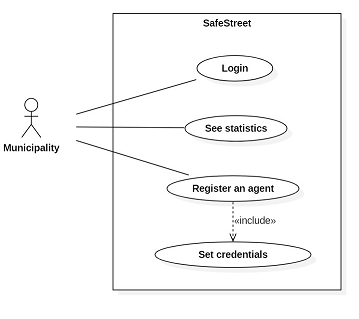
\includegraphics{Images/usecase_municipality.png}
\caption{\label{fig:MUC}Municipality Use Case }
\end{figure}
\begin{figure}[h]
\centering
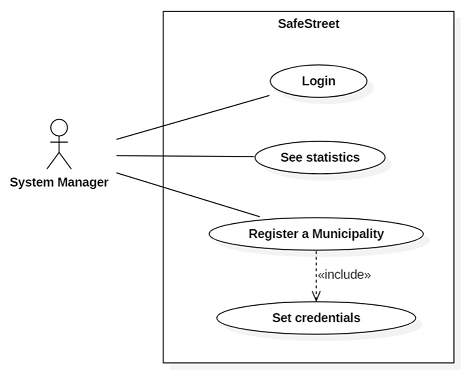
\includegraphics{Images/usecase_system_manager.png}
\caption{\label{fig:SMUC}System Manager Use Case }
\end{figure}
%.--------------------------------------------------------------------------------------------------------------------------------------------------------------
\subsubsection{Use Case Descriptions}
\begin{figure}[h]
\centering
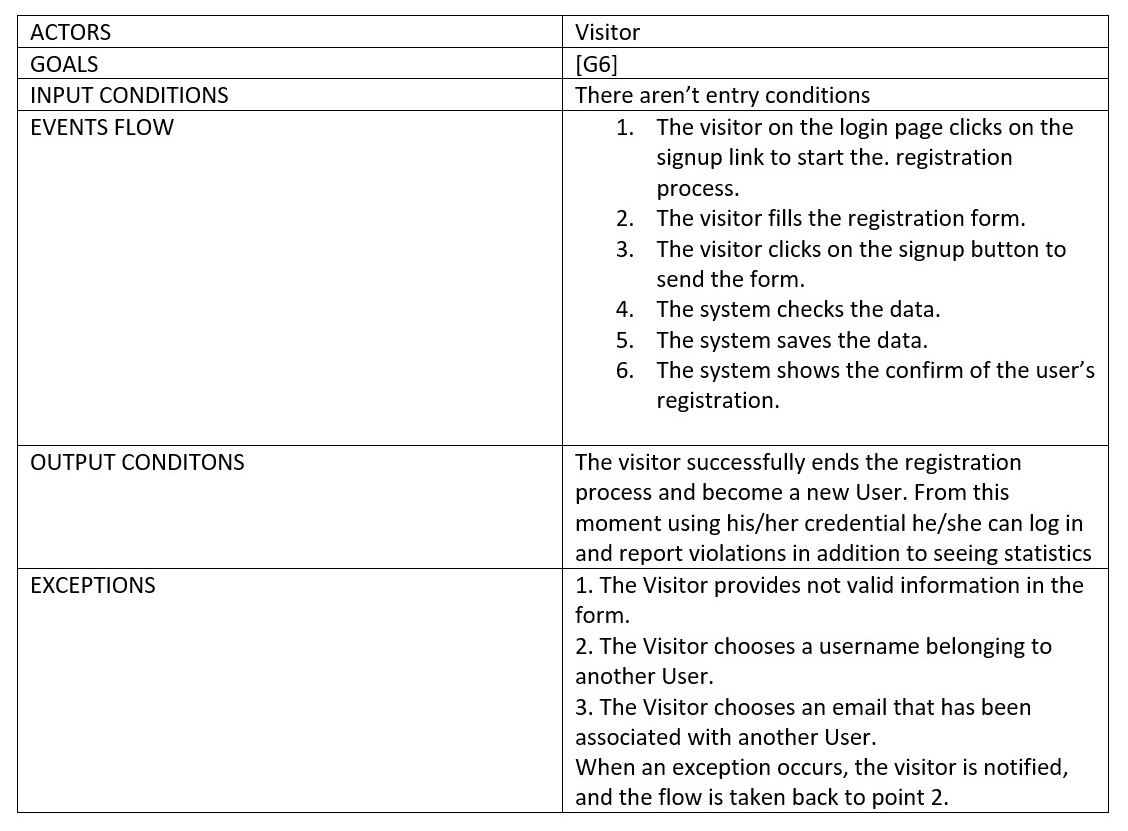
\includegraphics[width=\textwidth]{Images/visitor_use_case.png}
\caption{\label{fig:VUCD}Visitor Use Case Description}
\end{figure}
\begin{figure}[h]
\centering
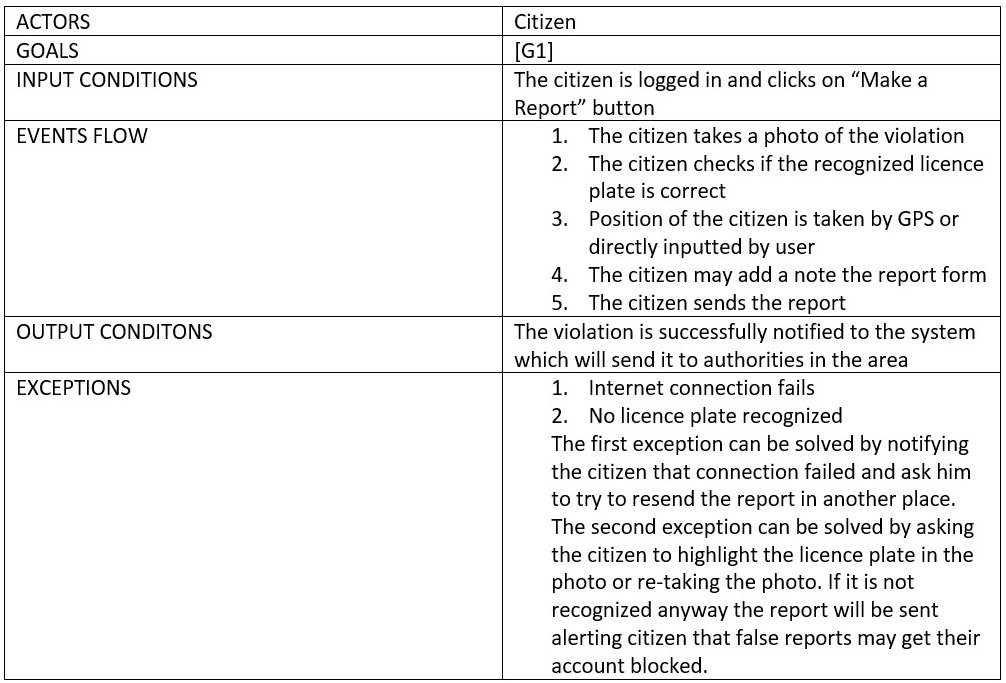
\includegraphics[width=\textwidth]{Images/citizen_use_case.png}
\caption{\label{fig:CUCD}Citizen Use Case Description }
\end{figure}
\begin{figure}[h]
\centering
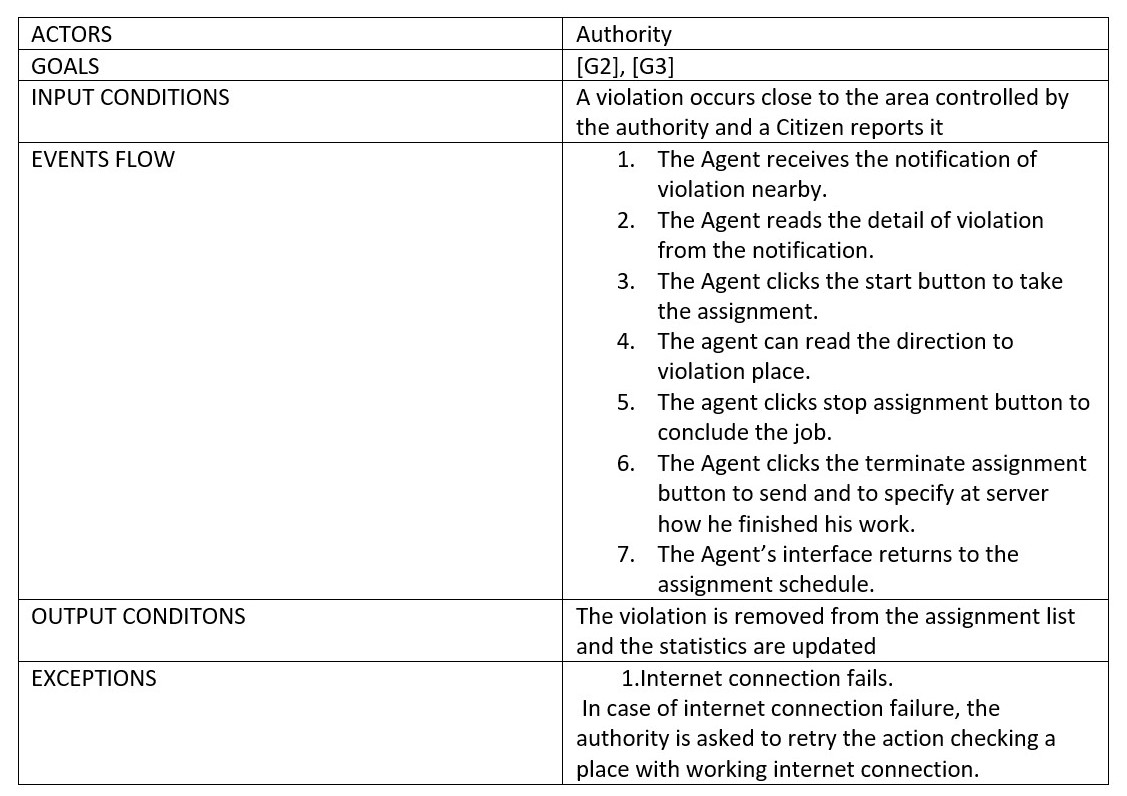
\includegraphics[width=\textwidth]{Images/authority_use_case.png}
\caption{\label{fig:AUCD}Authority Use Case Description 1}
\end{figure}
\begin{figure}[h]
\centering
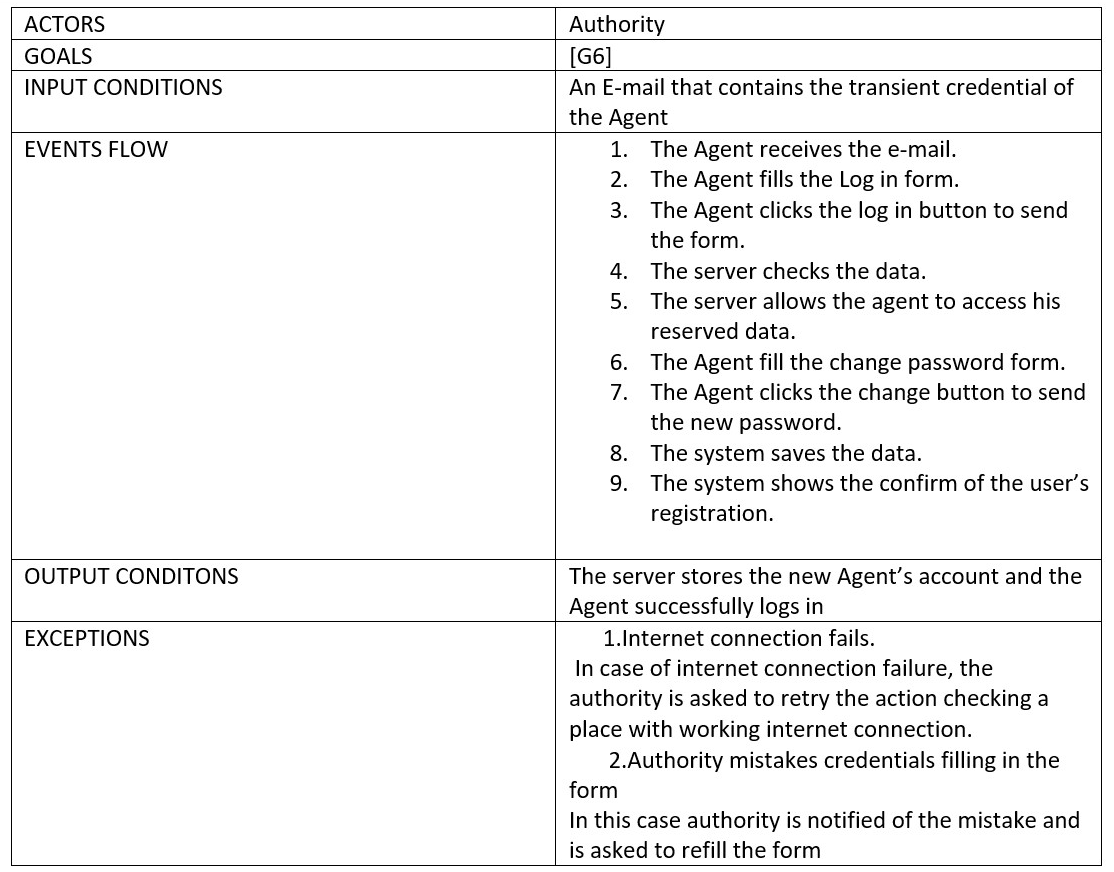
\includegraphics[width=\textwidth]{Images/authority_use_case2.png}
\caption{\label{fig:AUCD2}Authority Use Case Description 2}
\end{figure}
\begin{figure}[h]
\centering
\includegraphics[width=\textwidth]{Images/Municipality_use_case2.png}
\caption{\label{fig:MUCD}Municipality Use Case  Description 1}
\end{figure}
\begin{figure}[h]
\centering
\includegraphics[width=\textwidth]{Images/Municipality_use_case2.png}
\caption{\label{fig:MUCD2}Municipality Use Case  Description 2}
\end{figure}
\begin{figure}[h]
\centering
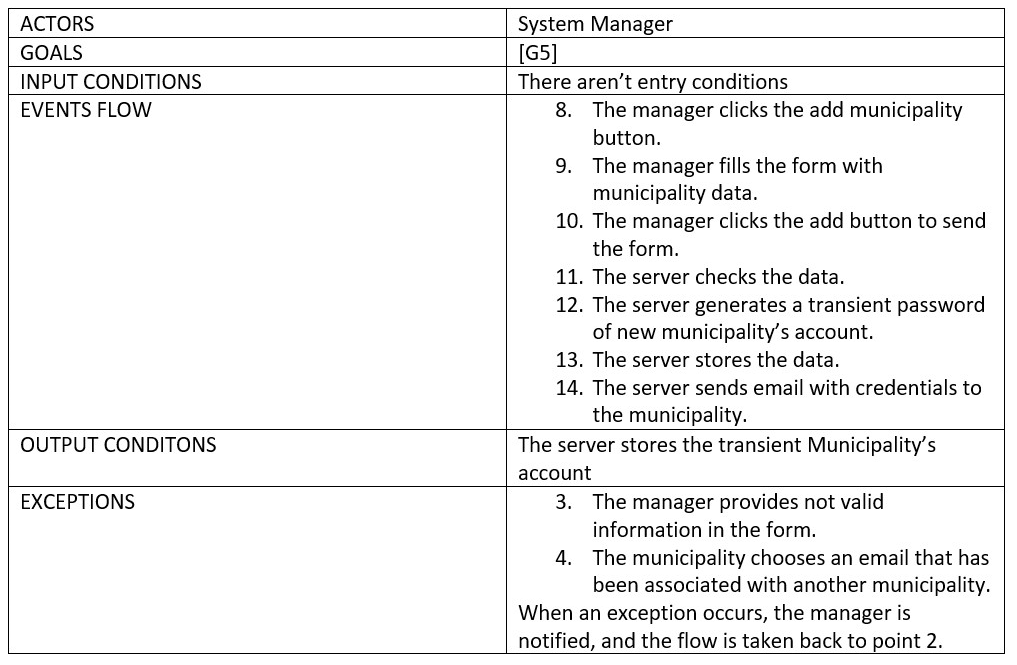
\includegraphics[width=\textwidth]{Images/system_manager_use_case.png}
\caption{\label{fig:SMUCD}System Manager Use Case  Description}
\end{figure}
\begin{figure}[h]
\centering
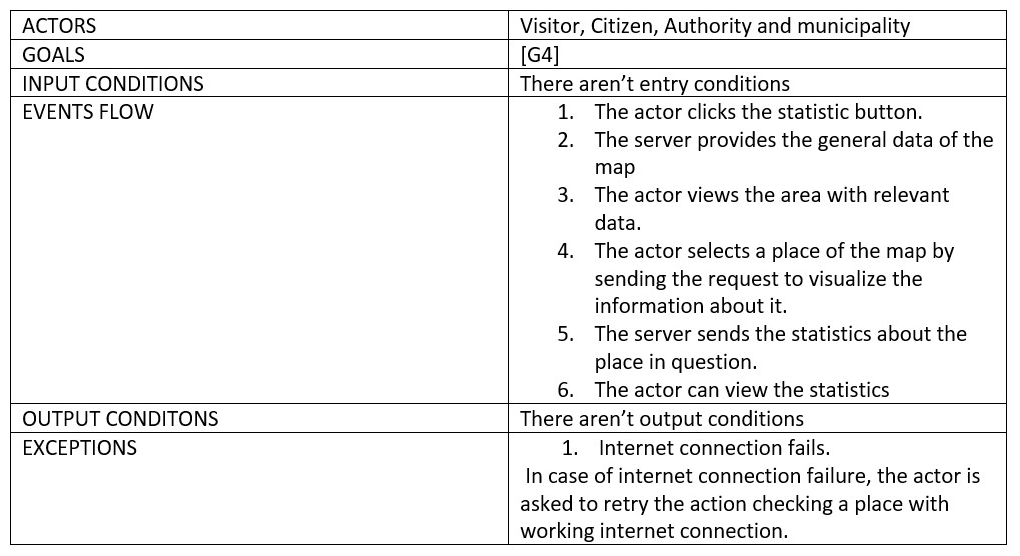
\includegraphics[width=\textwidth]{Images/common_use_case.png}
\caption{\label{fig:CUC}Common Use Case  Description 1} 
\end{figure}
\begin{figure}[h]
\centering
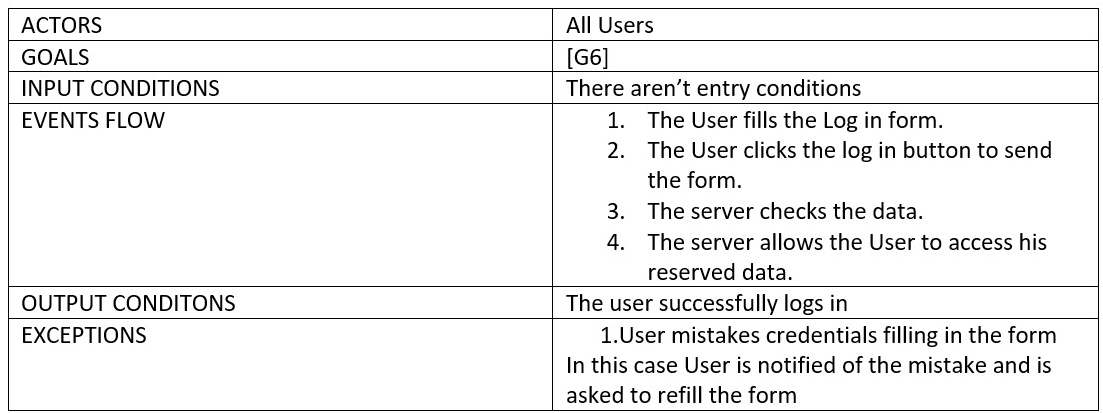
\includegraphics[width=\textwidth]{Images/common_use_case2.png}
\caption{\label{fig:CUC2}Common Use Case  Description 2}
\end{figure}
%.-------------------------------------------------------------------------------------------------------------------------------------------------------------
\subsubsection{Sequence  Diagrams}
\begin{figure}[h]
\centering
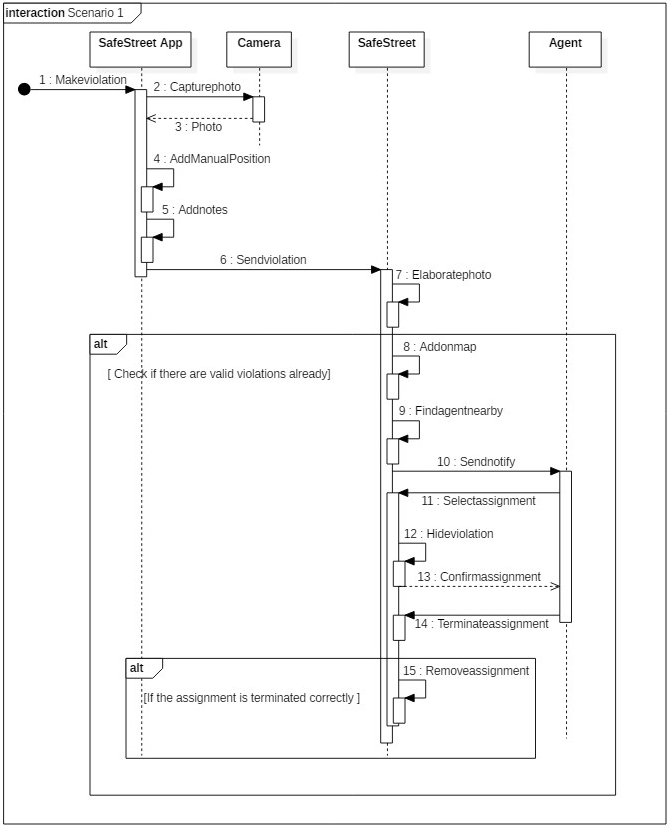
\includegraphics{Images/sequence_scenario1.png}
\caption{\label{fig:SDS1}Sequence Diagram Scenario 1}
\end{figure}
\begin{figure}[h]
\centering
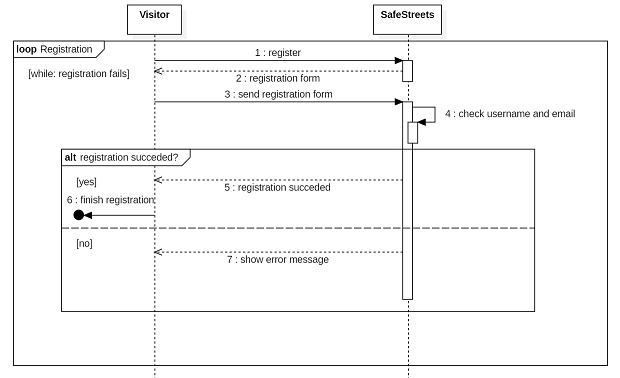
\includegraphics{Images/sequence_registration.png}
\caption{\label{fig:SR} Sequence Diagram Registration}
\end{figure}
\begin{figure}[h]
\centering
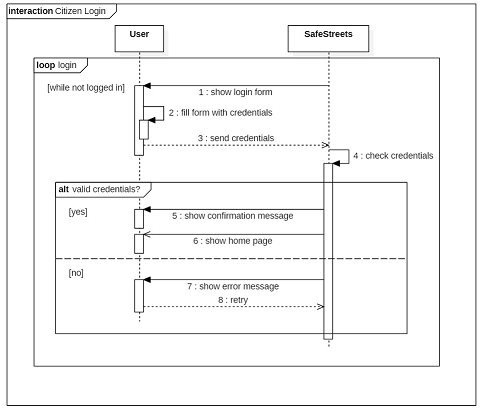
\includegraphics{Images/sequence_login.png}
\caption{\label{fig:SDL}Sequence Diagram Login}
\end{figure}
\begin{figure}[h]
\centering
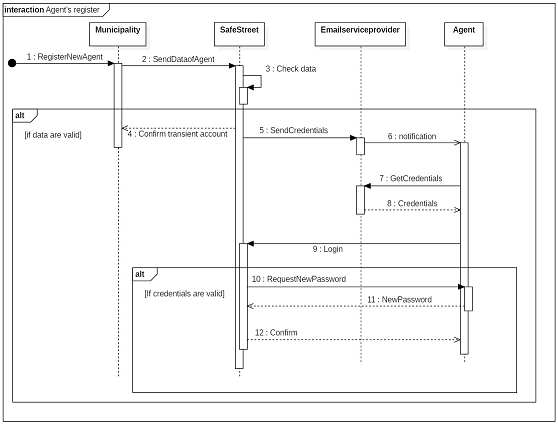
\includegraphics{Images/sequence_agent_register.png}
\caption{\label{fig:SDAR}Sequence Diagram Agent Registrtion} 
\end{figure}

%.-------------------------------------------------------------------------------------------------------------------------------------------------------------
\subsubsection{Mapping of Requirements and Domain Assumptions to their relative goal}
\begin{itemize}
\item G1) Notify authorities about traffic violations
\begin{itemize}
 \item R1) Authorities’ location must be known by the system when they are in service
 \item R2) When a Citizen makes a report the position is correctly added with the GPS when is available.
 \item R3) The right authorities are notified about violations.
 \item R10) When GPS is not available the user can input the position from a map.
 \item R11) Users to use the full service must be able to login providing the right credentials.
 \item D1) For each notification data and metadata provided by the system of the mobile phone are
correct.
 \item D3) GPS of authorities devices works correctly and gives the correct position every time.
 \item D4) Authorities if available correctly informs the system about their availability.
\end{itemize}
\item G2) Authorities must be able to take an available assignment
\begin{itemize}
 \item R1) Authorities’ location must be known by the system when they are in service.
 \item R3) The right authorities are notified about violations.
 \item R11) Users to use the full service must be able to login providing the right credentials.
 \item D3) GPS of authorities devices works correctly and gives the correct position every time.
 \item D4) Authorities if available correctly informs the system about their availability.
 \item D6) System Manager, Municipality and authorities respects their duty of care.
\end{itemize}
\item G3) Allow authorities to report a finished assignment
\begin{itemize}
 \item R4) Authority must be able to provide the system how the assignment finished: resolved and the
type of violation, no intervention needed when arrived, false report.
 \item R11) Users to use the full service must be able to login providing the right credentials.
 \item D6) System Manager, Municipality and authorities respects their duty of care
 \item D8) Information provided by authority are correct and no false report is ignored.
\end{itemize}
\item G4) Allow all actors to visualize updated statistics
\begin{itemize}
\item R5) The system must make Statistics available when asked.
\item R6) Statistics are always updated when an event happens.
 \item D8) Information provided by authority are correct and no false report is ignored.
\end{itemize}
\item G5) Allow the system manager to register Municipality to the service
\begin{itemize}
\item R7) For registering a Municipality his/hers data must be provided to a System manager who will add those data to the service to sign up him/her.
\item R9) When the creation of an account is successful the system must notify the Visitor sending an email to the address provided in the sign up process.
 \item R11) Users to use the full service must be able to login providing the right credentials.
\item D6) System Manager, Municipality and authorities respects their duty of care
\end{itemize}
\item G6) Allow a Visitor to join the system registering him/herself to ensure reliability of the information provided by him/her
\begin{itemize}
\item R8) A visitor must be able to begin sign up process in the SafeStreets App filling a form with his
data.
\item R9) When the creation of an account is successful the system must notify the Visitor sending an
email to the address provided in the sign up process.
 \item R11) Users to use the full service must be able to login providing the right credentials.
 \item R15) Each Username is unique
\end{itemize}
\item G7) Store information about violations provided by users:
\begin{itemize}
 \item R2) When a Citizen makes a report the position is correctly added with the GPS when is available.
 \item R4) Authority must be able to provide the system how the assignment finished: resolved and the
type of violation, no intervention needed when arrived, false report.
 \item R10) When GPS is not available the user can input the position from a map.
 \item R12) The camera of the mobile phone must be accessible to take photos of violations.
 \item R14) The User must be able to select the licence plate between the ones in output from the Licence
Plate Recognition algorithm.
 \item D8) Information provided by authority are correct and no false report is ignored.

\end{itemize}
\item G8) Identify potentially unsafe areas:
\begin{itemize}
\item R4) Authority must be able to provide the system how the assignment finished: resolved and the
type of violation, no intervention needed when arrived, false report.
\item R6) Statistics are always updated when an event happens.
\item D1) For each notification data and metadata provided by the system of the mobile phone are
correct
\item D8) Information provided by authority are correct and no false report is ignored.

\end{itemize}
\item G9) Allow municipality to register Authorities to the service
\begin{itemize}
\item R9) When the creation of an account is successful the system must notify the Visitor sending an
email to the address provided in the sign up process.
\item D6) System Manager, Municipality and authorities respects their duty of care
\item D7) When an authority is sent an email to register this will surely be received
\item D9) The Agent and municipality must be able to communicate
\item D10) Information of authority which is being registered are known by municipality
\end{itemize}
\item G10) Help the Municipality to make decision 
\begin{itemize}
\item R6) Statistics are always updated when an event happens.
\item R11) Users to use the full service must be able to login providing the right credentials.
\item R13) Suggestions must be available when municipalities request them.
\item D11) The data of external database are always available.
\end{itemize}
\end{itemize}

%.-------------------------------------------------------------------------------------------------------------------------------------------------------------
\subsection{Performance Requirements}
The system should be able to respond to a possibly great number of simultaneous requests. Based on 
data about Milan, there are over 100.000 parking violations a day, so the system should be able to keep 
track of at least 10 times that number of notifications a day. In some special cases, like public transport 
strikes, the number of violations could increase sensibly and the server could have to manage a lot of 
requests.

%.-------------------------------------------------------------------------------------------------------------------------------------------------------------
\subsection{Design Constraints}
%.-------------------------------------------------------------------------------------------------------------------------------------------------------------
\subsubsection{Standards compliance }
SafeStreets aims to become the smartest and quickest way to report violations in Italy. 
Nowadays, citizens who want to send a report can contact the authorities by calling an emergency number, 
but this can take a lot of time. Moreover, during critical events, phone lines could be unavailable. 
You can also use police website, but its interface is not user-friendly. In any case, you can’t send any 
evidence of the violation to the authorities. Anyway, the idea of our service is not unique: there are already 
similar services in other countries, like in India where there is “Public Eye. OFFICIAL BTP APP”.
%.-------------------------------------------------------------------------------------------------------------------------------------------------------------
\subsubsection{Hardware limitations}
\begin{itemize}
\item Mobile App
\begin{itemize}
\item Android smartphone
\item 2G/3G/4G connection
\item GPS
\end{itemize}
\item Web App
\begin{itemize}
\item Modern browser able to retrieve user's location
\end{itemize}
\end{itemize}
%.-------------------------------------------------------------------------------------------------------------------------------------------------------------
\subsection{Software System Attributes}
%.-------------------------------------------------------------------------------------------------------------------------------------------------------------
\subsubsection{Availability}
The system should be available 99,99\% of time. Considering only one State, there will be a time range 
in which notifications are considerably reduced (the night-time when citizen will less likely report 
a violation) and so reliability constraint for night-time could be reduced up to 99\% reducing also some 
resources allocated to the system.
%.-------------------------------------------------------------------------------------------------------------------------------------------------------------
\subsubsection{Reliability}
There are no strict costraints of Reliability if Availability costraints are respected
%.-------------------------------------------------------------------------------------------------------------------------------------------------------------
\subsubsection{Security}

Users credentials will be stored. Security of the data and of the communications user-system is a primary concern.

%.-------------------------------------------------------------------------------------------------------------------------------------------------------------
\subsubsection {Maintainability}
The system must be developed in a modular way so that new feature can be added.
Using a modular approach it is also possible to test the functionality of the single parts making it simpler to maintain.
Documentation must be also always updated in case of modifications of the system to always keep documentation aligned to the system.
%.-------------------------------------------------------------------------------------------------------------------------------------------------------------
\subsubsection{Scalability}
This system is designed to be optimized in Italy. It is possible to expand it later by choosing a more suitable
algorithm to recognize licence plates and by dividing computation of different states on different servers, so that reliability analysis made for Italy are still true for every single state. Information about boundaries
of states should be replicated in both states making the transition from one server to the other smoother.
%.-------------------------------------------------------------------------------------------------------------------------------------------------------------
\subsubsection{Accuracy}
Accuracy of the position of authorities and violations has to be the best possible. All the sensors used must provide positions' data with an error lower than 20 meters. We can consider a larger bound of accuracy because authorities work on a given area so from a well taken photo, they should be able to recognize the place of the violation even if the position given by the GPS is not too accurate.












%------------------------------------------------------------------------------------------------------------------------------------------------
\clearpage
{\color{Blue}{\section{Formal Analysis Using Alloy}}}
\label{sect:alloy}
%.-------------------------------------------------------------------------------------------------------------------------------------------------------------
\subsection{Alloy Model Description}
The main goal of SafeStreets is to increase safety on the streets and, in order to reach this goal, it is important
that every report made by Citizens is taken care as fast as possible by authorities. We have modelled
a goal stating that every agent must be working on an assignment if he/she is not already dealing with
another. In the model there are only the entities that are relevant to that goal and simplification about
users’ location are made to make it more understandable. In addition, to make sure that our model
with domain assumptions and requirements makes it possible to reach the goal we set, we have also checked how different worlds may be generated and that some borderline cases aren’t ignored.

%.-------------------------------------------------------------------------------------------------------------------------------------------------------------
\subsection{Alloy Model}
\lstinputlisting[language=alloy]{Files/model.als}

%.-------------------------------------------------------------------------------------------------------------------------------------------------------------
\newpage
\subsection{Results}
\begin{figure}[h]
\centering
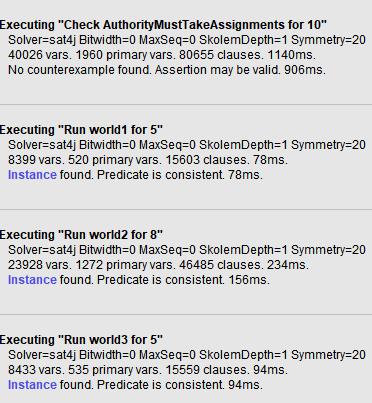
\includegraphics[width=\textwidth]{Images/alexecutionstatus.png}
\caption{Result}
\end{figure}
\begin{figure}[h]
\centering
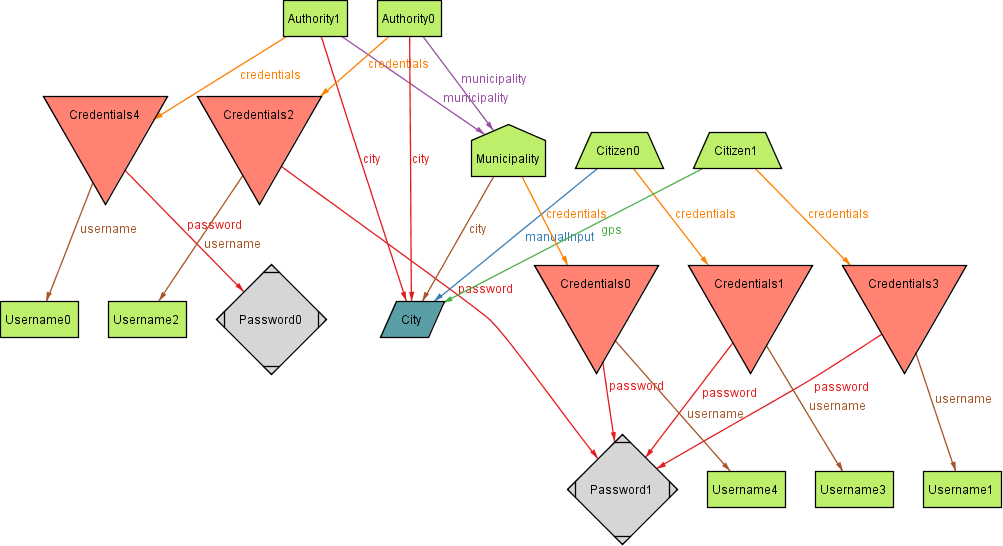
\includegraphics[width=\textwidth]{Images/alworld1.png}
\caption{First world}
\textbf{This world represents the borderline case in which no notification are present and so no assignment is associated to authorities , there are neighter statistics nor suggestions}
\end{figure}
\begin{figure}[h]
\centering
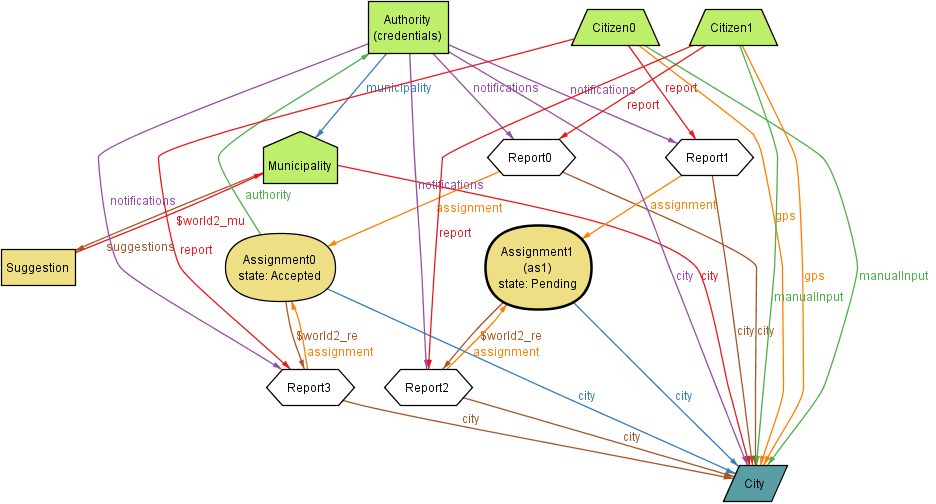
\includegraphics[width=\textwidth]{Images/alworld2.png}
\caption{Second world}
\textbf{This world represent the case in which no assignment is completed and so no statistics are available
Credentials are projected away for the sake of clarity.
}
\end{figure}
\begin{figure}[h]
\centering
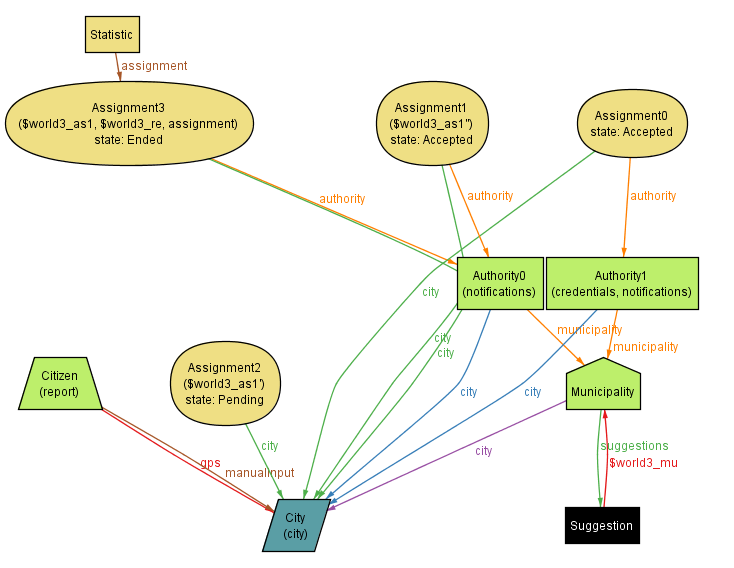
\includegraphics[width=\textwidth]{Images/alworld3.png}
\caption{Third world}
\textbf{This world represents a more generic world where assignments pending,accepted,finished are all generated.
Also here credentials are projected away for the sake of clarity.}
\end{figure}




%------------------------------------------------------------------------------------------------------------------------------------------------
\clearpage
{\color{Blue}{\section{Effort Spent}}}
\label{sect:effort}
\begin{figure}[h]
\centering
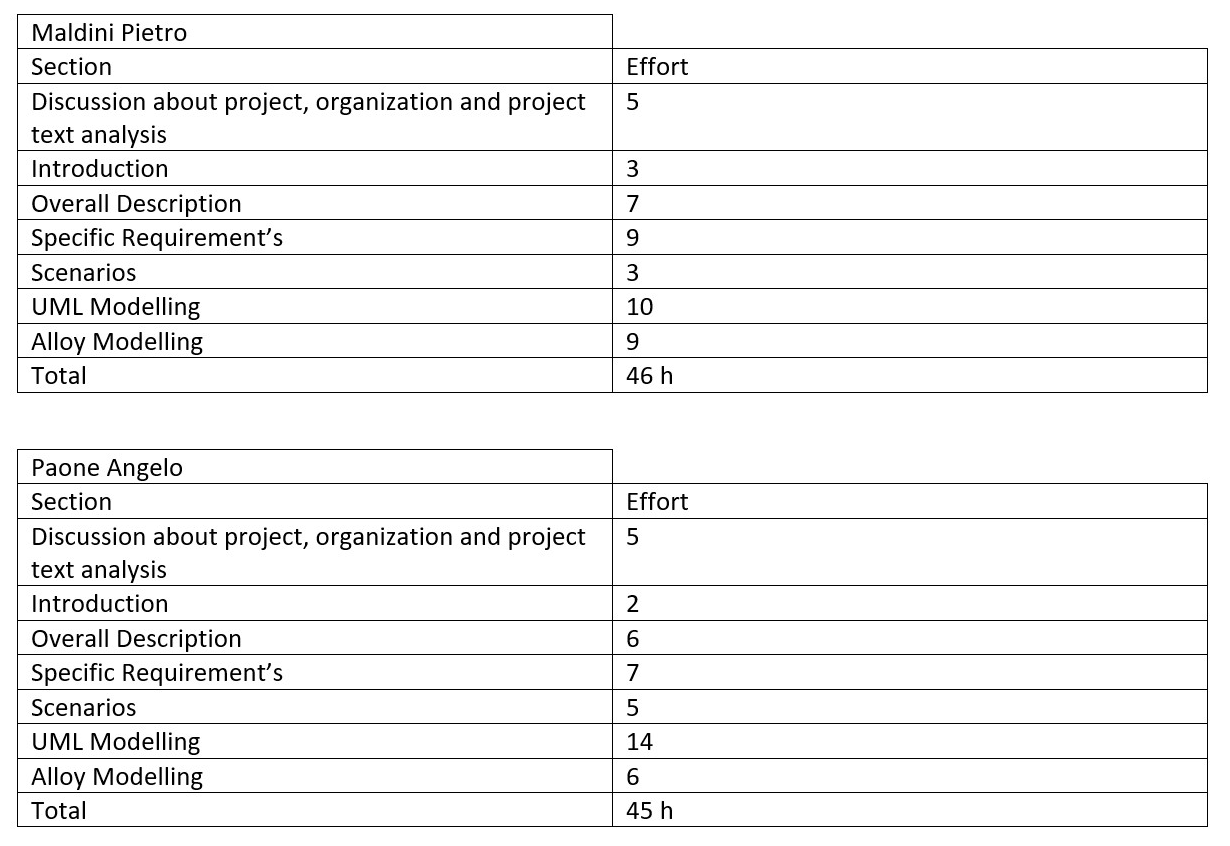
\includegraphics[width=\textwidth]{Images/effort.png}
\end{figure}


%------------------------------------------------------------------------------------------------------------------------------------------------
\clearpage
{\color{Blue}{\section{References}}}
\label{sect:effort}
\begin{itemize}

\item \href{https://www.gps.gov/systems/gps/performance/accuracy/}{GPS Performances}

\item	\href{https://milano.corriere.it/notizie/cronaca/18_dicembre_12/milano-allarme-sosta-selvaggia-ogni-giorno-divieto-centomila-auto-solo-3percento-sanzioni-abe397ce-fe44-11e8-89a1-ceb28fd9db2c.shtml?refresh_ce-cp TODO when everything else is done}{article about traffic violations in milan}

\item Vliet, Hans : van copertina Software engineering : principles and practice 2008

\item 	Pressman, Roger S. Principi di ingegneria del software 2004



\end{itemize}
%------------------------------------------------------------------------------------------------------------------------------------------------




\end{document}
